\documentclass[]{BasiliskReportMemo}
\usepackage{AVS}

\newcommand{\submiterInstitute}{Autonomous Vehicle Simulation (AVS) Laboratory,\\ University of Colorado}

\newcommand{\ModuleName}{extPulsedTorque}
\newcommand{\subject}{Module to apply a cyclic pulsed disturbance torque}
\newcommand{\status}{First Version}
\newcommand{\preparer}{H. Schaub}
\newcommand{\summary}{This module allows the user to setup a cyclic pulsed external disturbance torque.  The pulses are symmetrically applying $\pm\bm\tau_{pulsed}$ followed by a specified off period before repeating.     }


\begin{document}


\makeCover


%
%	enter the revision documentation here
%	to add more lines, copy the table entry and the \hline, and paste after the current entry.
%
\pagestyle{empty}
{\renewcommand{\arraystretch}{1.1}
\noindent
\begin{longtable}{|p{0.5in}|p{4.5in}|p{1.14in}|}
\hline
{\bfseries Rev}: & {\bfseries Change Description} & {\bfseries By} \\
\hline
v1.0 & Initial document & H. Schaub \\
\hline

\end{longtable}
}

\newpage
\setcounter{page}{1}
\pagestyle{fancy}

\tableofcontents
~\\ \hrule ~\\


\begin{figure}[htb]
	\centerline{
	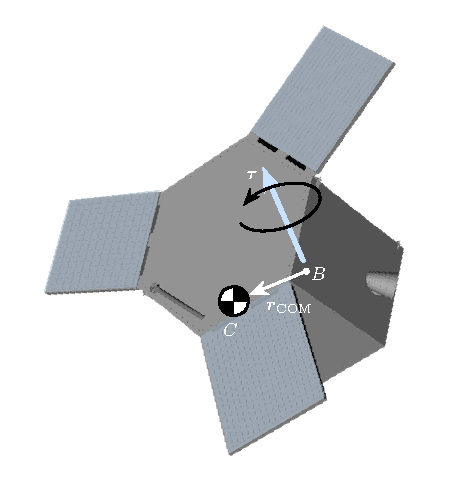
\includegraphics[]{Figures/TorqueDiagram1}
	}
	\caption{Illustration of Disturbance Torque acting on a rigid body}
	\label{fig:extPulse1}
\end{figure}
\section{Introduction}
This module allows a special pulsed external disturbance torque $\bm \tau$ to be applied onto a rigid body.   The torque is taken about the body-fixed point $B$, and the vector components are given in the body frame $\mathcal{B}$ as illustrated in Figure~\ref{fig:extPulse1}.  



\begin{figure}[htb]
	\centerline{
	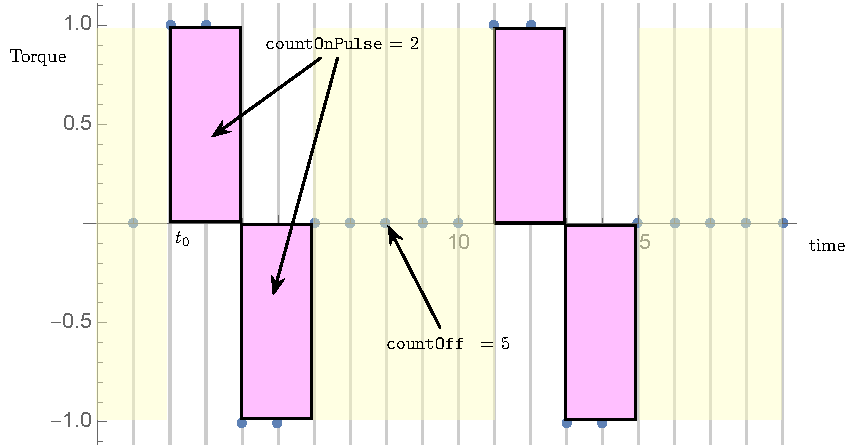
\includegraphics[]{Figures/TorqueDiagram2}
	}
	\caption{Illustration of Pulsed Disturbance Torque }
	\label{fig:extPulse2}
\end{figure}
\section{Specifying the Pulsed Disturbance Torque}
The module creates a cyclic disturbance torque which is applied to the rigid body.  The torque vector $\bm\tau$ is applied for equal time periods as $+\bm\tau$ and $-\bm\tau$.  This is followed by a specified off period before repeating.  This pattern is illustrated in Figure~\ref{fig:extPulse2}.  

Note that the pulse and off periods are specified through integer counts of the simulation integration time.




\section{Module Parameters}
The external disturbance torque vector and pulsing parameters are set directly from python.  

\subsection{{\tt pulsedTorqueExternalPntB\_B} Parameter}
This vector sets the external torque, about point $B$, in $\mathcal{B}$ body-frame vector components.

\subsection{{\tt countOnPulse} Parameter}
This integer represents the duration of both the $+\bm\tau$ and $-\bm\tau$ pulses.  The integer value represents how many integration time steps the pulse is on.

\subsection{{\tt countOff} Parameter}
This integer represents the off period duration between $\pm$ pulsing.  The integer value represents how many integration time steps the pulse is off.





\end{document}
